\documentclass[11pt, oneside]{article} 
\usepackage{geometry}
\geometry{letterpaper} 
\usepackage{graphicx}
	
\usepackage{amssymb}
\usepackage{amsmath}
\usepackage{parskip}
\usepackage{color}
\usepackage{hyperref}

\graphicspath{{/Users/telliott_admin/Tex/png/}}
% \begin{center} 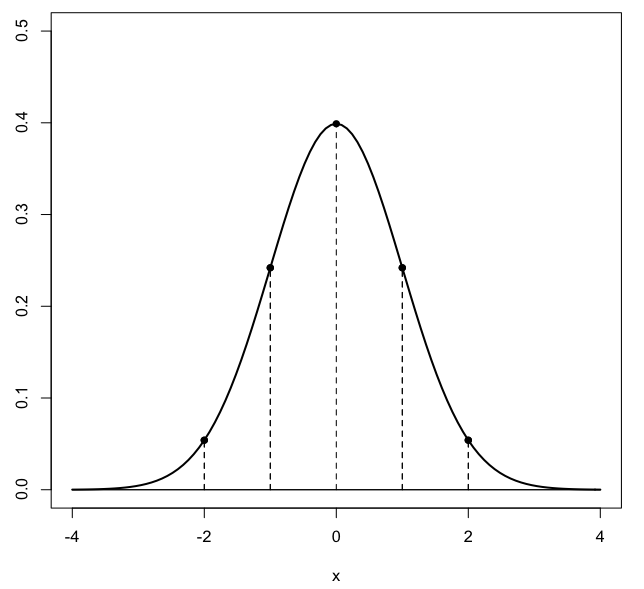
\includegraphics [scale=0.4] {gauss3.png} \end{center}

\title{Surface normal}
\date{}

\begin{document}
\maketitle
\Large
\subsection*{n dS six ways}

A characteristic feature of vector calculus for physics is that we seem to do everything twice, first in $\mathbb{R}^2$ and then again, in $\mathbb{R}^3$.

My experience has been that $\mathbb{R}^2$ is easy and $\mathbb{R}^3$ is hard, even though already in $\mathbb{R}^2$ we have the ideas of multivariable calculus, line integrals, and even the 2D versions of curl and divergence.

One difference is that we have not just Cartesian but cylindrical and spherical coordinates in $\mathbb{R}^3$.  Another even bigger difference is that for some problems, we will substitute surface integrals for line integrals.  For example, we will often want to compute 
\[ \mathbf{F} \cdot \mathbf{\hat{n}} \ dS \]
for some surface.  

The second term above ($\mathbf{\hat{n}} \ dS$) is the surface area element as a vector in the direction normal (perpendicular) to the surface, at that point.  For problem solving, it is crucial to have a solid understanding of how to derive $\mathbf{\hat{n}} \ dS$ for various geometries or types of coordinates, as well as what it signifies.

In general, one can always find two vectors parallel to the surface
\begin{center} 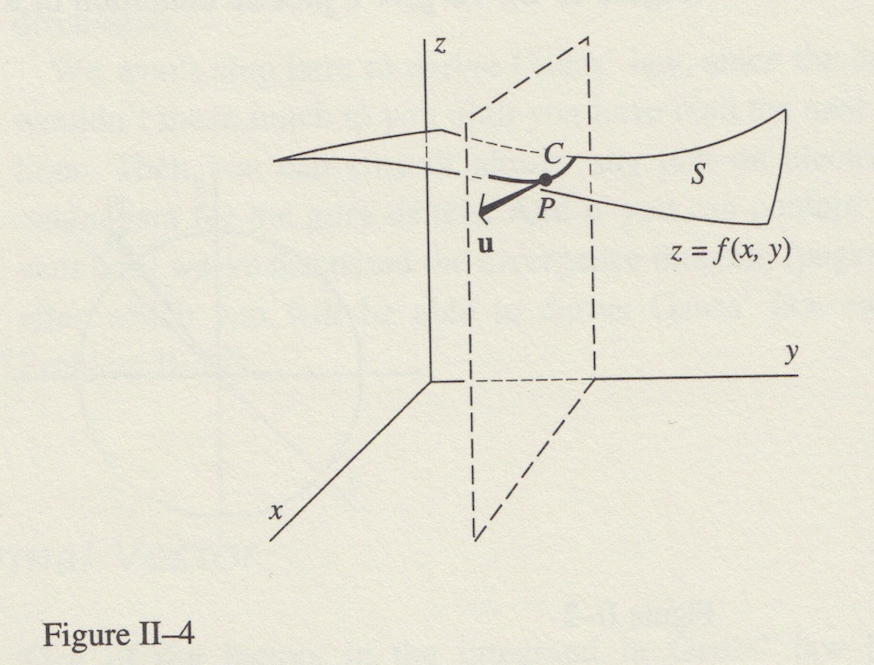
\includegraphics [scale=0.3] {intersect.png} \end{center}
namely, $\langle 1, 0, f_x \rangle$ and $\langle 0, 1, f_y \rangle$, and then form their cross-product.  But some geometries have symmetry that allow us to avoid that.

\subsection*{plane}
In the $xy$-plane things are really easy.  The normal vector points straight up.  It is $\hat{\mathbf{k}}$ or
\[ \hat{\mathbf{n}} = \ \langle 0,0,1 \rangle \]
Similarly, the surface element is just $dA$, so we have
\[ \hat{\mathbf{n}} \ dS = \ \langle 0,0,1 \rangle  \ dx \ dy \]

\subsection*{cylinder}
On the surface of a cylinder oriented along the $z$ axis, the normal vector points straight out radially (no $z$ component).  If we look down from the top at the circular cross-section, the normal vector points out with components 
\[ \mathbf{n} = \langle x,y,0 \rangle \]
The length of $\mathbf{n}$ is $a$, the radius of the cylinder, so
\[ \hat{\mathbf{n}} = \frac{1}{a} \ \langle x,y,0 \rangle \]

The vertical side of the surface area element is just $\Delta z$, while in the horizontal direction it is $r$ or $a$ times $\Delta \theta$, thus 
\[ \Delta S = a \ \Delta \theta \ \Delta z \]
\[ dS = a \ d \theta \ dz \]
\[ \hat{\mathbf{n}} \ dS = \ \langle x,y,0 \rangle  \ d \theta \ dz \]
Although it seems weird to mix $x,y$ with $\theta$, the idea is to keep things like this until we do the dot product with the field as will usually happen.

\subsection*{sphere}
On the surface of a sphere, the normal vector again points straight out.  It is
\[ \mathbf{n} = \langle x,y,z \rangle \]
as we've seen before.  If the sphere has radius $a$, then the length of $\mathbf{n}$ is $a$, and
\[ \hat{\mathbf{n}} = \frac{1}{a} \ \langle x,y,z \rangle \]
The surface of the sphere is parametrized by just $\phi$ and $\theta$ (no $r$ since it is fixed with $r=a$).  

Looking down at the horizontal circular cross-section for a given $\phi$, the radius of that circle is $a \sin \phi$, so the horizontal component of the surface area element is $a \sin \phi \ \Delta \theta$.  The vertical component is a great circle (radius $r = a$), so its length is just $a \ \Delta \phi$.

\[ \Delta S = a^2 \ \sin \phi \ \Delta \phi \ \Delta \theta \]
\[ dS = a^2 \ \sin \phi \ d \phi \ d \theta \]
Let's just check:
\[ \int dS = \int_0^{2 \pi} \int_0^{\pi} a^2 \ \sin \phi \ d \phi \ d \theta \]
\[ = 2 \pi a^2  \int_0^{\pi} \ \sin \phi \ d \phi \]
\[ = 2 \pi a^2 \ [ \ - \cos \phi  \ \bigg |_0^{\pi} \ ] \]
\[ = 4 \pi a^2 \]
and
\[ \hat{\mathbf{n}} \ dS = a \ \langle x,y,z \rangle   \ \sin \phi \ d \phi \ d \theta \]

Very quickly, what we have here is $a^2 \ \sin \phi \ d \phi \ d \theta$ times the unit normal, which is $ \langle x,y,z \rangle/a$, and that accounts for the single power of $a$ in the result.

\subsection*{graph of a function}
If our surface is the graph of a function $g(x,y)$ then we can just remember the formula
\[ \hat{\mathbf{n}} \ dS = \ \langle -f_x,-f_y,1 \rangle  \ dx \ dy  \]

If we forget and need to work it out, the deal is that we get a linear approximation to the plane surface using $f_x$ and $f_y$ so that
\[ \mathbf{u} = \langle 1,0,f_x \rangle \ dx \]
\[ \mathbf{v} = \langle 0,1,f_y \rangle \ dy \]

The cross-product $\mathbf{u} \times \mathbf{v}$ gives 
\[ \mathbf{n} = \ \langle -f_x,-f_y,1 \rangle  \]
\begin{center} 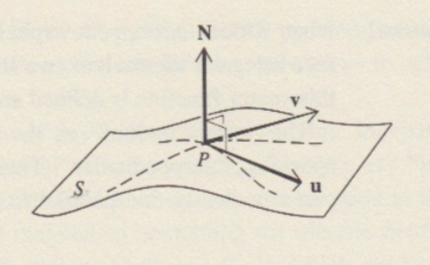
\includegraphics [scale=0.4] {n=uxv.png} \end{center}
Note that the part of $\mathbf{n}$ in the $\mathbf{\hat{k}}$ direction is just $1$.

As usual, the length of $\mathbf{n} $ is
\[ |\mathbf{n}| = \sqrt{f_x^2 + f_y^2 + 1} \]
but we won't need this because it will cancel.  

Just write
\[ \hat{\mathbf{n}} = \frac{\mathbf{n}}{|\mathbf{n}|} = \ \frac{\langle -f_x,-f_y,1 \rangle}{n}  \]

$dS$ is larger than its shadow in the $xy$-plane by exactly this same factor
\[ dS \ \cos \theta = dA \]
where 
\[\cos \theta = \frac{\mathbf{n} \cdot \hat{\mathbf{k}} }{|\mathbf{n}| \ |\mathbf{k}|} \]
\[ =  \frac{1}{|\mathbf{n}| \ |\mathbf{k}|} \]
\[ = \frac{1}{|\mathbf{n}|} \]
Hence
\[ \hat{\mathbf{n}} \ dS =  \hat{\mathbf{n}} \ \frac{1}{\cos \theta} \ dA = \ \frac{\langle -f_x,-f_y,1  \rangle}{n} \ n \ dA \]
\[ = \ \langle -f_x,-f_y,1 \rangle \ dA  \]
\[ = \ \langle -f_x,-f_y,1 \rangle  \ dx \ dy  \]
Depending on whether $\mathbf{n}$ points up or down we may change the sign.

\subsection*{parametrization (parameterization)}
More generally, we may have only a parametrization of the surface (it's not an explicit function $f(x,y)$).
\[ S =
\left\{
	\begin{array}{l}
		x  = x(u,v)  \\
		y  = y(u,v)  \\
		z  = z(u,v)
	\end{array}
\right.
\]
Then
\[ \hat{\mathbf{n}} \ dS = | \mathbf{r_u} \times \mathbf{r_v} | \ du \ dv \]

\subsection*{normal vector}
Auroux has a last example, in which we only know a normal vector $\mathbf{N}$ to the surface $S$.  Examples include a plane 
\[ ax + by + cz = d  \]
\[ \mathbf{N} = \ \langle a,b,c> \]
or $S$ is given by 
\[ g(x,y,z) = 0 \]
\[ \mathbf{N} = \nabla g \]
Then
\[ dS = \frac{1}{\cos \theta} \ dA = \frac{|\mathbf{N}|}{\mathbf{N} \cdot \hat{\mathbf{k}}} \ dA \]
\[ \hat{\mathbf{n}} \ dS  = \frac{|\mathbf{N}| \ \hat{\mathbf{n}}}{\mathbf{N} \cdot \hat{\mathbf{k}}} \ dA \]
As Auroux says, what happens if I take the unit normal $\mathbf{n}$, and I multiply it by the length of my other normal $|\mathbf{N}|$?  It's just $\mathbf{N}$.
\[ \hat{\mathbf{n}} \ dS  = \frac{\mathbf{N}}{\mathbf{N} \cdot \hat{\mathbf{k}}} \ dA \]
And again, this is "within sign", depending on how $\hat{\mathbf{n}}$ is oriented.



\end{document}  